\documentclass{../llncs}
%%%%%%%%%%%%%%%%%%%%%%%%%%%%%%%%%%%%%%%%%%%%%%%%%%%%%%%%%%%
%% package sillabazione italiana e uso lettere accentate
\usepackage[latin1]{inputenc}
\usepackage[english]{babel}
\usepackage[T1]{fontenc}
%%%%%%%%%%%%%%%%%%%%%%%%%%%%%%%%%%%%%%%%%%%%%%%%%%%%%%%%%%%%%

% https://en.wikibooks.org/wiki/LaTeX/Source_Code_Listings
%%%%%%%%%%%%%%%%%%%%%%%%%%%%
\usepackage{listings}

\usepackage{xcolor}
\definecolor{darkgreen}{HTML}{007700}

\lstdefinestyle{style_qa}{
basicstyle=\small\ttfamily, columns=fullflexible,
keywordstyle=\color{violet}\bfseries, commentstyle=\color{darkgreen},
language=C++, breaklines=true,	 % sets automatic line breaking
captionpos=b,					 % sets the caption-position to bottom
morekeywords={Plan,System,Event,Dispatch,Context,ip,host,port,-httpserver,QActor,context,
normal,switchTo,transition,whenMsg,finally,repeatPlan,stopAfter,resumeLastPlan,
onMsg,addRule,replyToCaller,onEvent,removeRule,javaRun,whenTime,sendto,emit,else,not,selfMsg},
stringstyle=\color{blue},     	 % string literal style
caption={\lstname},
% title=\lstname,                  % show the filename of files included with \lstinputlisting; also try caption instead of title
numbers=left, numberstyle=\tiny,
stepnumber=1, numbersep=5pt, frame=shadowbox % , float=*
}

\lstnewenvironment{codice_qa}[1][]
{\lstset{style=style_qa, #1}}{}

% \begin{lstlisting}
% ...
% \end{lstlisting}

% \begin{codice_qa}[caption={Programma Blink, "Hello World!"}]
% ...
% \end{codice_qa}

% \lstinputlisting[language=Python, firstline=37, lastline=45]{source_filename.py}
% \lstinputlisting[style=style_qa]{code/robotClient.qa}
%%%%%%%%%%%%%%%%%%%%%%%%%%%%

\usepackage{url}
\usepackage{xspace}
\usepackage{color}
\makeatletter
%%%%%%%%%%%%%%%%%%%%%%%%%%%%%% User specified LaTeX commands.
\usepackage{../manifest}

\makeatother


%%%%%%%
 \newif\ifpdf
 \ifx\pdfoutput\undefined
 \pdffalse % we are not running PDFLaTeX
 \else
 \pdfoutput=1 % we are running PDFLaTeX
 \pdftrue
 \fi
%%%%%%%
 \ifpdf
 \usepackage[pdftex]{graphicx}
 \else
 \usepackage{graphicx}
 \fi
%%%%%%%%%%%%%%%
 \ifpdf
 \DeclareGraphicsExtensions{.pdf, .jpg, .tif}
 \else
 \DeclareGraphicsExtensions{.eps, .jpg}
 \fi
%%%%%%%%%%%%%%%

\newcommand{\java}{\textsf{Java}}
\newcommand{\android}{\texttt{Android}}
\newcommand{\dsl}{\texttt{DSL}}
\newcommand{\jazz}{\texttt{Jazz}}
\newcommand{\rtc}{\texttt{RTC}}
\newcommand{\ide}{\texttt{Contact-ide}}
\newcommand{\xtext}{\texttt{XText}}
\newcommand{\xpand}{\texttt{Xpand}}
\newcommand{\xtend}{\texttt{Xtend}}
\newcommand{\pojo}{\texttt{POJO}}
\newcommand{\junit}{\texttt{JUnit}}

\newcommand{\action}[1]{\texttt{#1}\xspace}
\newcommand{\codescript}[1]{{\scriptsize{\texttt{#1}}}\xspace}
\newcommand{\code}[1]{{\color{blue}\small{\texttt{#1}}}}
\newcommand{\fname}[1]{{\small{\color{magenta}\texttt{#1}}}}
\newcommand{\node}{\textsf{NodeJs}}
\newcommand{\qa}{\textsf{\textit{QActor}}}

% Cross-referencing
\newcommand{\labelsec}[1]{\label{sec:#1}}
\newcommand{\xs}[1]{\sectionname~\ref{sec:#1}}
\newcommand{\xsp}[1]{\sectionname~\ref{sec:#1} \onpagename~\pageref{sec:#1}}
\newcommand{\labelssec}[1]{\label{ssec:#1}}
\newcommand{\xss}[1]{\subsectionname~\ref{ssec:#1}}
\newcommand{\xssp}[1]{\subsectionname~\ref{ssec:#1} \onpagename~\pageref{ssec:#1}}
\newcommand{\labelsssec}[1]{\label{sssec:#1}}
\newcommand{\xsss}[1]{\subsectionname~\ref{sssec:#1}}
\newcommand{\xsssp}[1]{\subsectionname~\ref{sssec:#1} \onpagename~\pageref{sssec:#1}}
\newcommand{\labelfig}[1]{\label{fig:#1}}
\newcommand{\xf}[1]{\figurename~\ref{fig:#1}}
\newcommand{\xfp}[1]{\figurename~\ref{fig:#1} \onpagename~\pageref{fig:#1}}
\newcommand{\labeltab}[1]{\label{tab:#1}}
\newcommand{\xt}[1]{\tablename~\ref{tab:#1}}
\newcommand{\xtp}[1]{\tablename~\ref{tab:#1} \onpagename~\pageref{tab:#1}}
% Category Names
\newcommand{\sectionname}{Section}
\newcommand{\subsectionname}{Subsection}
\newcommand{\sectionsname}{Sections}
\newcommand{\subsectionsname}{Subsections}
\newcommand{\secname}{\sectionname}
\newcommand{\ssecname}{\subsectionname}
\newcommand{\secsname}{\sectionsname}
\newcommand{\ssecsname}{\subsectionsname}
\newcommand{\onpagename}{on page}

\newcommand{\xauthA}{Filippo Frabetti}
\newcommand{\xauthB}{Nicola Semprini}
\newcommand{\xauthC}{Paolo Magnani}
\newcommand{\xfaculty}{II Faculty of Engineering}
\newcommand{\xunibo}{Alma Mater Studiorum -- University of Bologna}
\newcommand{\xaddrBO}{viale Risorgimento 2}
\newcommand{\xaddrCE}{via Venezia 52}
\newcommand{\xcityBO}{40136 Bologna, Italy}
\newcommand{\xcityCE}{47023 Cesena, Italy}

%
% Comments
%
\newcommand{\todo}[1]{\bf{TODO:}\emph{#1}}


\begin{document}

\title{Software Engineering process template (initial) }

\author{\xauthA, \xauthB, \xauthC}

\institute{%
  \xunibo\\\xaddrBO, \xcityBO\\\email{filippo.frabetti@studio.unibo.it}
}

\maketitle

\begin{abstract}
\footnotesize
(This part is optional)
%%This a Latex template to be used for the explicit representation of the production process adopted in the Software Systems Engineering course. 
THIS DOCUMENT MUST FILL AT MOST TWO PAGES AND MUST BE PRINTED ON A SINGLE PAPER SHEET.

The document can be compiled by using the \fname{kitISLatex.zip} given in \code{iss2018/it.unibo.issMaterial/issdocs/Lab}
  
\keywords{
(This part is optional)
Software engineering, software development process, process representation, .... }
\end{abstract}

\sloppy

%===========================================================================
\section{Introduction}
\labelsec{intro}
%===========================================================================

%===========================================================================
\section{Vision}
\labelsec{vision}
%=========================================================================== 
 
%===========================================================================
\section{Requirements}
\labelsec{Requirements}

%With reference to a \texttt{mbot} physical robot working in a virtual environment, build an application that sends the data sensed by the virtual and the real sonars to the radar. More specifically:
%\begin{itemize}
%\item[-]the data of the \emph{virtual sonar} \texttt{sonar1} must be displayed on the direction of angle=\fname{30};
%\item[-]the data of the \emph{virtual sonar} \texttt{sonar2} must be displayed on the direction of angle=\fname{120};
%\item[-]the data of the \emph{virtual sonar} on the virtual robot must be displayed on the direction of angle=\fname{90} at the fixed distance of \fname{40};
%\item[-]the data of the \emph{real sonar} on the physical robot must be displayed on the direction of angle=\fname{0};
%\end{itemize}

% 13 - A new problem
\begin{enumerate}
\item The physical robot must expose in a visible way a \code{Led} and:
\begin{itemize}
\item[-] the Led must be \code{on} when the robot is engaged by an user (human or machine);
\item[-] the Led must be \code{off} when the robot is available for booking.
\end{itemize}
\item the robot system does not expose any public available usage interface;
\item in order to use the robot, an user must first of all send 'to the system' a \code{booking request}. The system
must return an answer including an \code{access token} if the robot is available. If the answer is negative, (robot
already engaged) and the request includes a '\texttt{notify-me flag}', the system must notify the user when to robot
becomes again available;
\item the user that receives the \code{access token} must send within a given \code{acquisition-deadline} (e.g. \code{30 sec}) the request for a \emph{robot-driving command interface}, by appending to the request the \code{access token}. If the
\emph{acquisition-deadline} expires, the robot returns in its 'available state';
\item the user can use the \emph{robot-driving command interface} at most for a prefixed \code{usage-duration} time;
\item the user can explicitly release the robot resource by sending a \code{booking release} message;
\item if many users attempt to book the robot resource 'at the same time', the system could operate in two different
ways:
\begin{itemize}
\item[(a)] by selecting the first \emph{emitted} request;
\item[(b)] by selecting the first \emph{received} request
\end{itemize}
\end{enumerate}
%===========================================================================

%===========================================================================
\section{Requirement analysis}
\labelsec{ReqAnalysis}
%===========================================================================
% 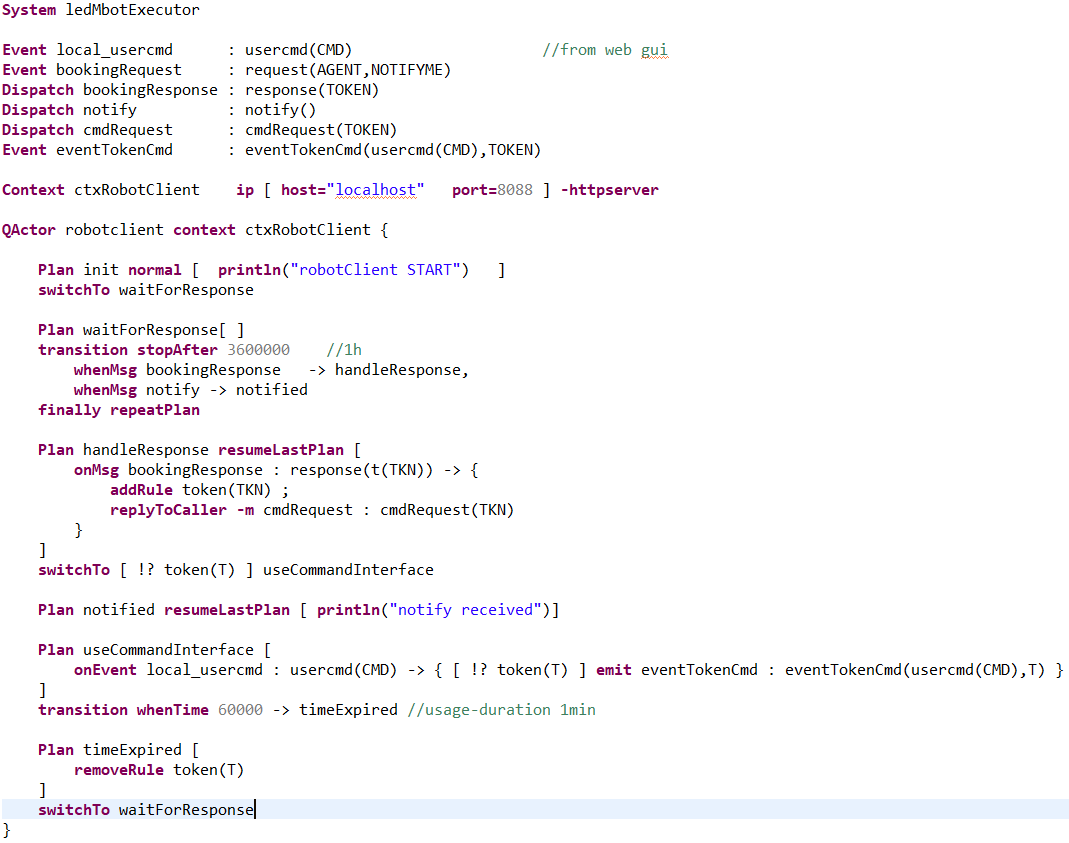
\includegraphics[scale = 0.4]{img/req1.png}
\lstinputlisting[style=style_qa]{robotClient.qa}

%===========================================================================
\section{Problem analysis}
\labelsec{ProblemAnalysis}
%===========================================================================
% 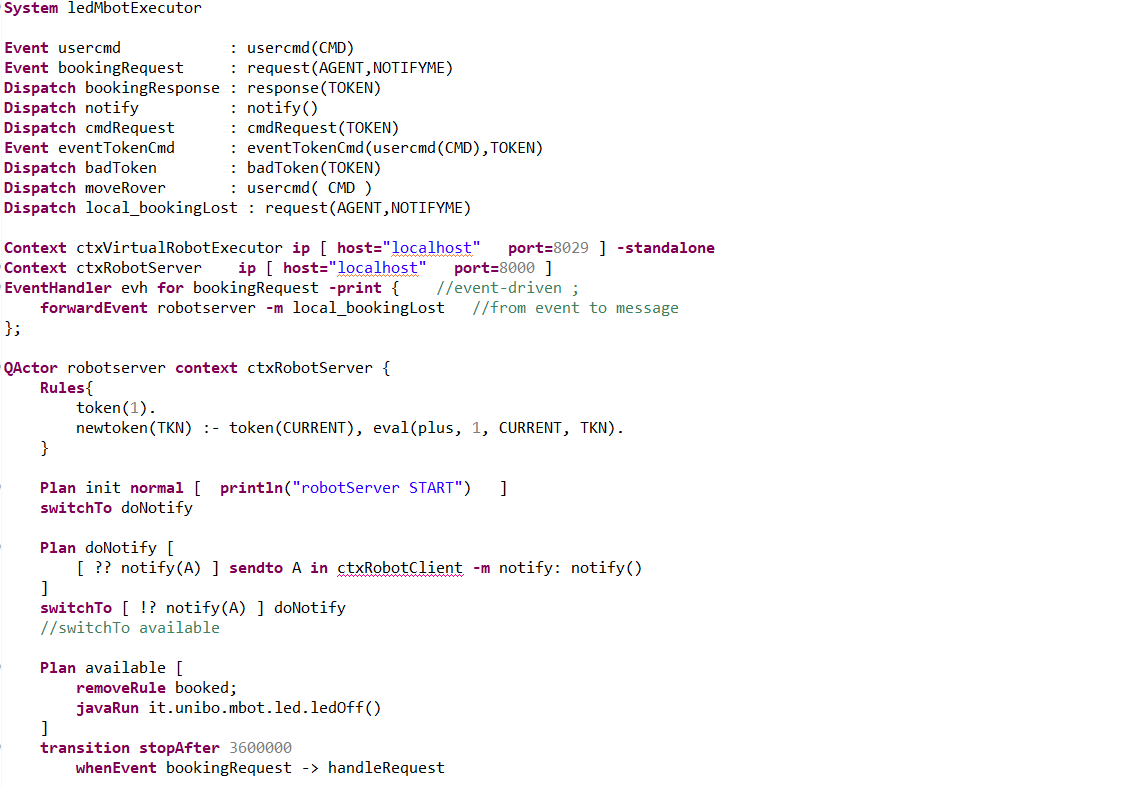
\includegraphics[scale = 0.4]{img/probA1.png}
% 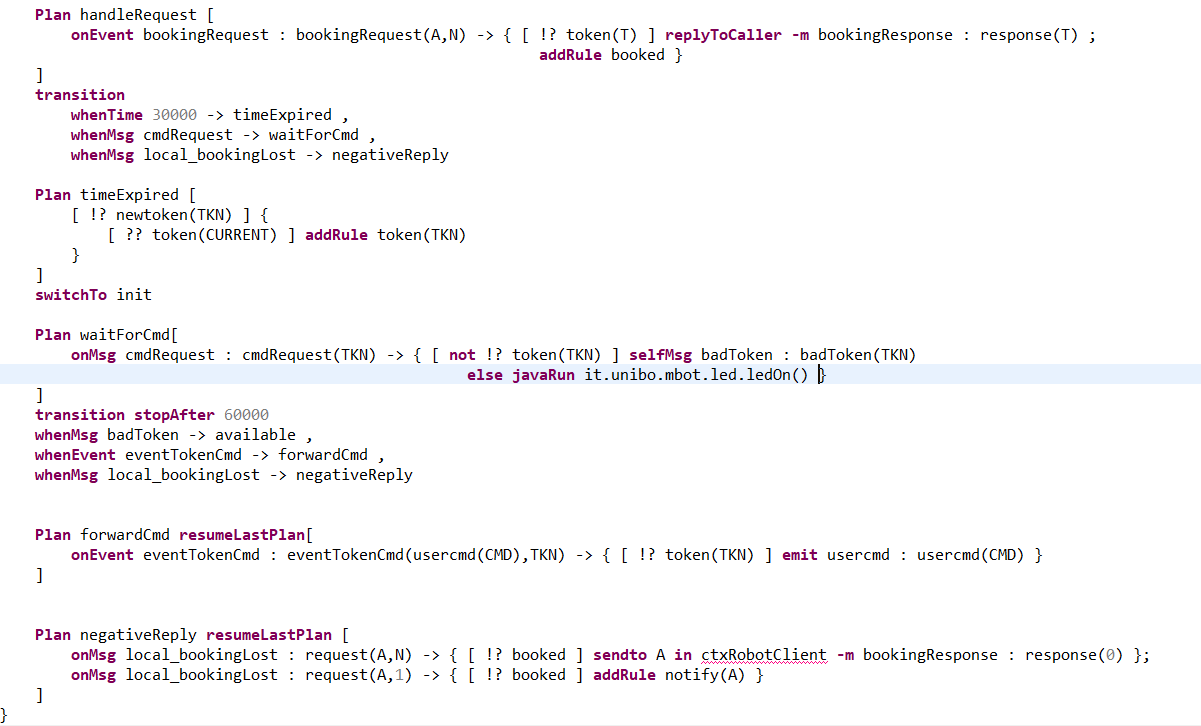
\includegraphics[scale = 0.4]{img/probA2.png}
\lstinputlisting[style=style_qa]{robotServer.qa}

%===========================================================================
\section{Project}
\labelsec{Project}
%===========================================================================

%===========================================================================
\section{Implementation}
\labelsec{Implementation}
%===========================================================================

%===========================================================================
\section{Testing}
\labelsec{Testing}
%===========================================================================

%===========================================================================
\section{Maintenance}
\labelsec{Maintenance}
%===========================================================================

%===========================================================================
\section{Deployment}
\labelsec{Deployment}
%===========================================================================
 
%===========================================================================
\section{Author}
\labelsec{Author}
%===========================================================================

\vskip.5cm
%%% \begin{figure}
\begin{tabular}{ | c |  }
\hline
  % after \\: \hline or \cline{col1-col2} \cline{col3-col4} ...
  Photo of the author 
  \\
\hline
   %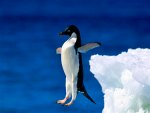
\includegraphics[scale = 0.7]{img/foto_autore.jpg}
   %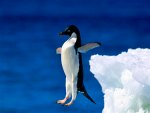
\includegraphics{img/foto_autore.jpg}
  \\
\hline
\end{tabular}
 
\end{document}












